\documentclass[a4paper]{article}

\usepackage[a4paper,margin=3.5cm]{geometry}
\usepackage{cancel}
\usepackage{tikz}
\usepackage{amsmath,amsfonts,amssymb}
\usepackage{xcolor}
\usepackage{tcolorbox}
\usepackage{polynom}
\usepackage{wrapfig}
\usepackage{booktabs}
\usepackage{tabularx}
\usepackage{multicol}
\usepackage{hyperref}
\usepackage[ngerman]{babel}
\usepackage{tikz}
\usepackage{pgfplots}
\pgfplotsset{compat=1.18}
\usepackage{pstricks}
\usepackage{pst-plot}
\usepackage{textcomp}
\usepackage{import}
\usepackage{pdfpages}
%\usepackage{transparent}


\newcommand{\incfig}[2][1]{%
    \def\svgwidth{#1\columnwidth}
    \import{./figures/}{#2.pdf_tex}
}

\setlength{\parindent}{0pt}

\newcommand{\tbox}[2][0.8\linewidth]{
    \begin{center}
        \begin{tcolorbox}[colback=white, colframe=gray, width=#1]
                #2
        \end{tcolorbox}
    \end{center}}

\newcommand{\regel}[2][0.8\linewidth]{
    \begin{center}
        \begin{tcolorbox}[title=regel, colback=white, colframe=blue, width=#1]
                #2
        \end{tcolorbox}
    \end{center}}

\newcommand{\nt}[2][0.9\linewidth]{
    \begin{center}
        \begin{tcolorbox}[title=Notitz:, colback=white, colframe=gray, width=#1]
                #2
        \end{tcolorbox}
    \end{center}}


\newcommand{\ex}[2][\linewidth]{
    \begin{center}
        \begin{tcolorbox}[title=Beispiel:, colback=white, colframe=brown, width=#1]
                  #2
        \end{tcolorbox}
    \end{center}}


\newcommand{\q}[2][\linewidth]{
    \begin{center}
        \begin{tcolorbox}[title=Frage:, colback=white, colframe=purple, width=#1]
                  #2
        \end{tcolorbox}
    \end{center}}

\usepackage{titlesec}

\titleformat{\section}{\normalfont\Large\bfseries}{\thesection}{1em}{}[\vspace{0.5ex}]


\title{Untersuchung der Kraftwirkung zwischen zwei elektrisch geladenen Kugeln}
\author{Daniel Renschler}
\date{}

\begin{document}
\maketitle


\section{Ziel des Versuchs}
\label{ssub:Ziel des Versuchs}
Beantworten Der Forschungsfrage:


\begin{tcolorbox}[colback=black!5!white,colframe=black!75!black,title=Forschungsfrage]
  Gilt für die Konstante~$\epsilon_0$ in der Gleichung 
  \begin{align}
  F_{el} = \dfrac{1}{4\pi\epsilon_0} \cdot \dfrac{q_1 \cdot q_2}{r^2} \label{coloumb}
  \end{align}
  der Zusammenhang
  \begin{align}
  c^2 = \dfrac{1}{\epsilon_0 \cdot \mu_0} \text{?}\label{halt-c}
  \end{align}
\end{tcolorbox}

\section{Thematischer Kontext und ggf. die zu überprüfenden Behauptungen}
Im Rahmen dieses Versuchs soll die Forschungsfrage überprüft werden, ob der
Zusammenhang $c^2 = \frac{1}{\epsilon_0 \cdot \mu_0}$ gilt, wobei $\epsilon_0$
die elektrische Feldkonstante und $\mu_0$ die magnetische Feldkonstante
darstellen. Dies wird mithilfe der Coulombschen Kraft, die in Gleichung
(\ref{coloumb}) beschrieben wird, untersucht. Der Versuch zielt darauf ab, die
Beziehung zwischen den Konstanten $\epsilon_0$ und $\mu_0$ zu untersuchen und
somit grundlegende Kenntnisse der Elektromagnetismus-Theorie zu vertiefen.



\section{Ort und Zeit der Durchführung, Namen der Experimentatoren} % (fold)
\label{ssub:Ort und Zeit der Durchführung, Namen der Experimentatoren}
Der Versuch wurde in Raum 349 der Rolf Benz Schule in Nagold am Freitag, dem
10. Februar durchgeführt. Experimentator war Daniel Renschler.



\section{Beschreibung und ggf. Abbildung des Versuchsaufbau} % (fold)
\label{ssub:Beschreibung und ggf. Abbildung des Versuchsaufbau}
Der Versuch wurde in einer Simulation durchgeführt die uns bereitgestellt
wurde \footnote{https://phet.colorado.edu/sims/html/coulombs-law/latest/coulombs-law-en.html}.
Bei dem Versuch sind zwei Geladene Teilchen, die einen Abstand voneinander
haben. In der Simulation kann man den Abstand einstellen ud welche Ladung sie haben sollen.
Für den Veruch wurde folgendes Verwendet: Ladung 1 = 7 µC, Ladung 2 = 5 µC und einen Abstand von 3cm.
Daraus Resultierte eine Kraft von 349,516N mit der Sich die Teilchen beeinflussen.

\begin{figure}[htpb]
  \begin{center}
    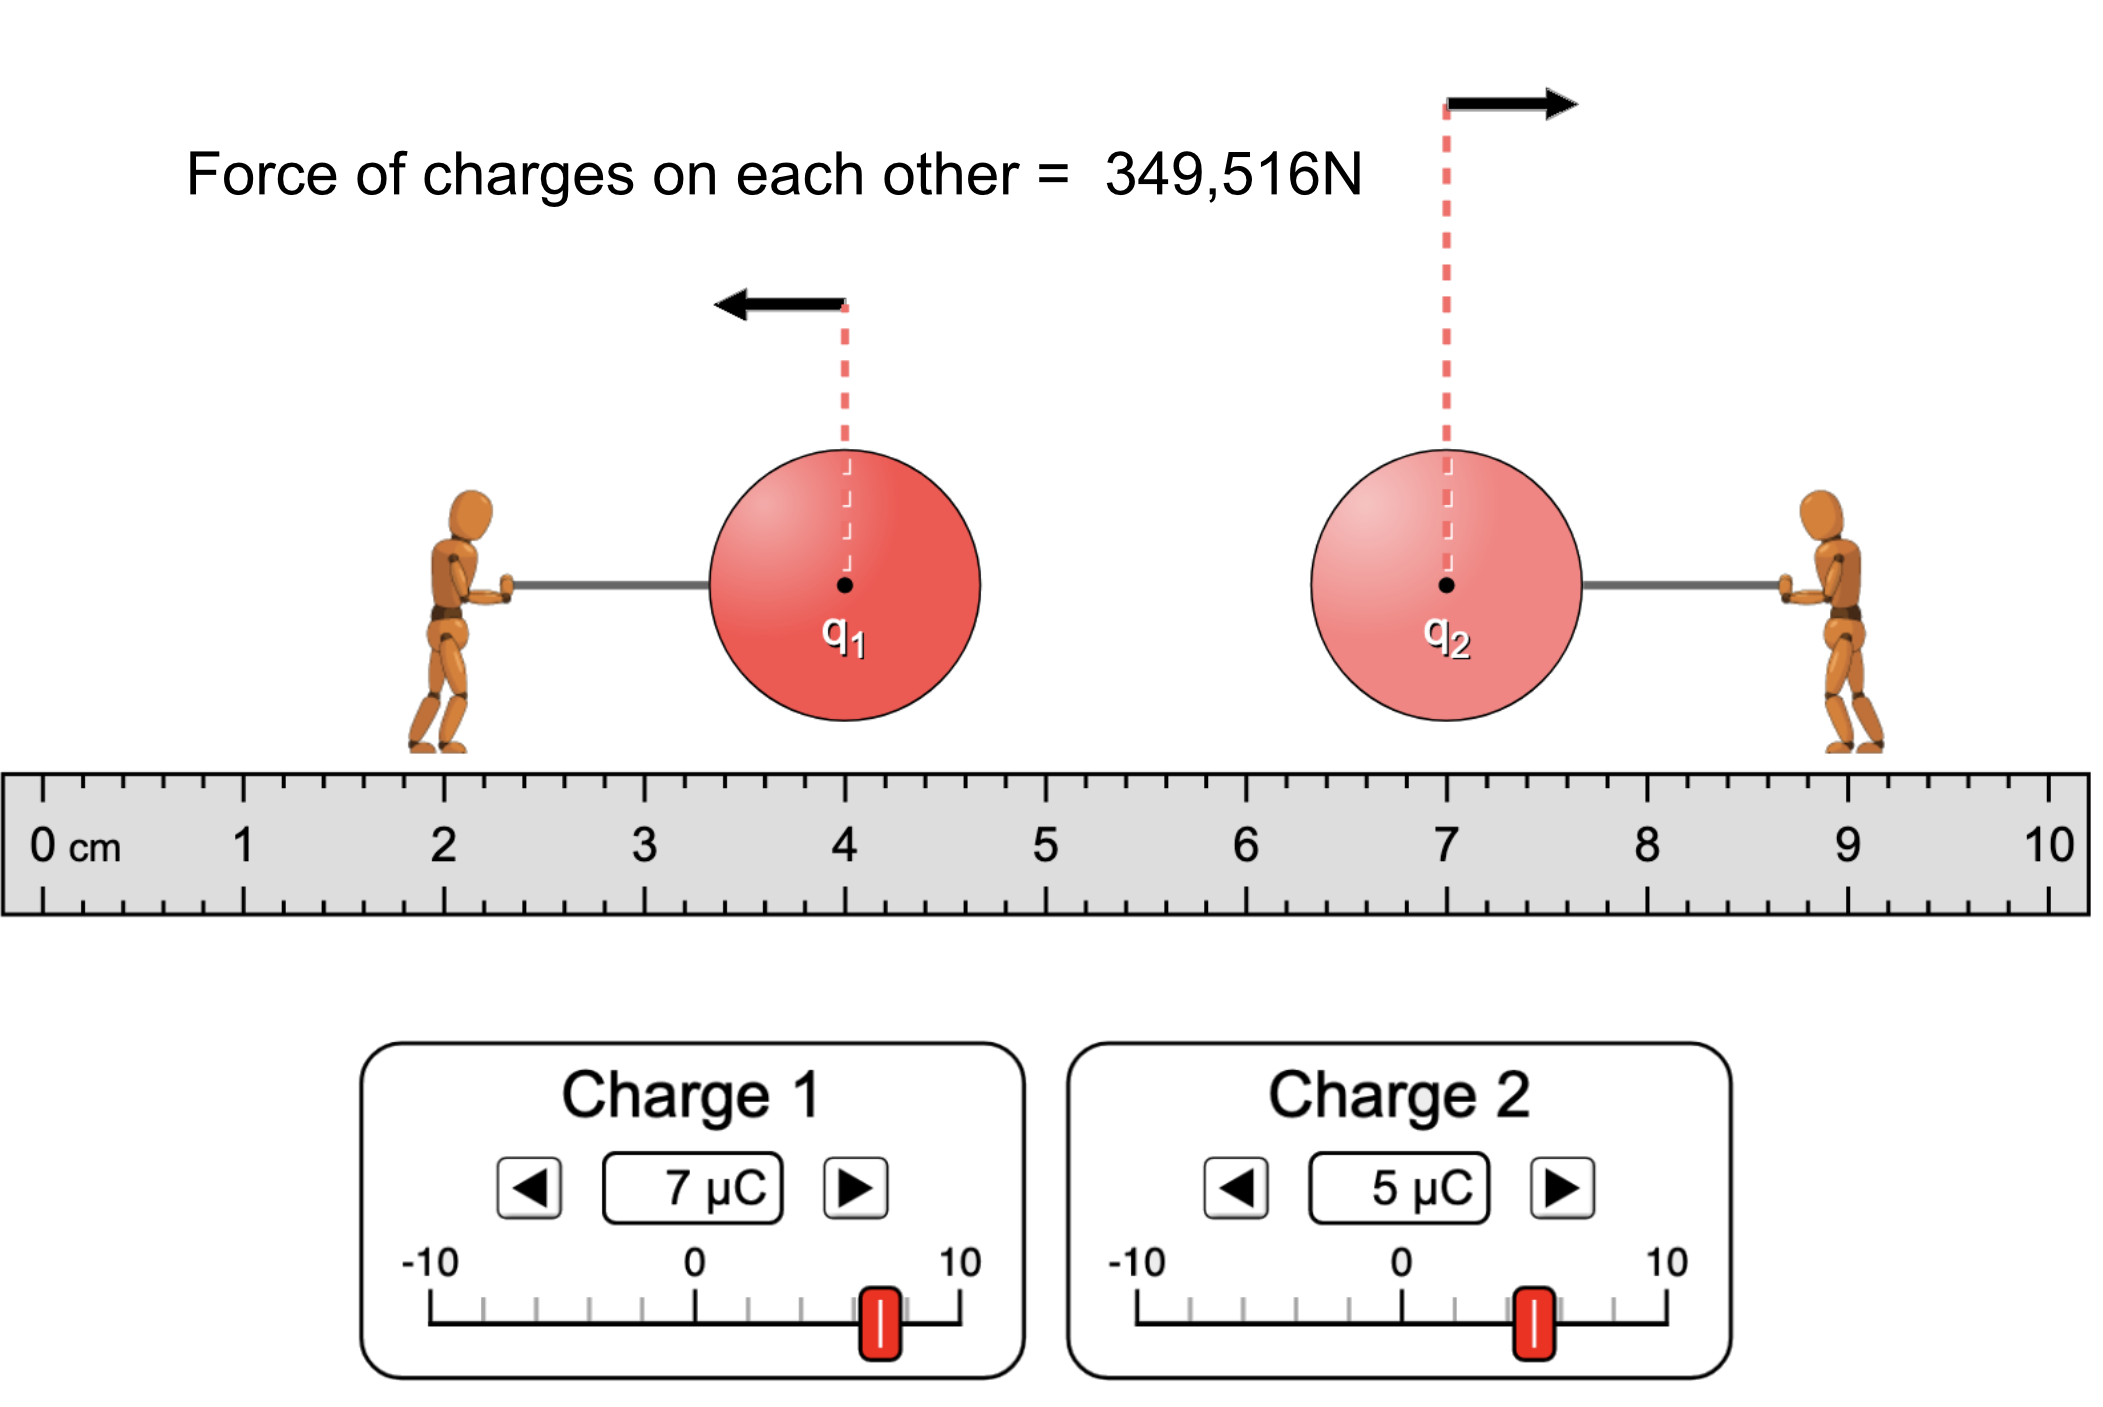
\includegraphics[width=0.5\textwidth]{simu-1.png}
  \end{center}
  \caption{Simulation-coloumb}
  \label{fig:simulation}
\end{figure}


\section{Beschreibung der Versuchsdurchführung} % (fold)
\label{ssub:Beschreibung der Versuchsdurchführung}
Die Versuchsdurchführung wurde schon großteils erläutert, Werte wurden in der
Simulation eingestellt und eine Kraft ist daraus resultiert, mit dieser kann
man dann weiterrechnen.

\section{Messergebnisse und Auswertung}
\subsection{Versuch 1}

In der Ersten Tabelle, dem ersten Versuch sind die gegebenen Bedingungen
Abstand $r$ der Mittelpunkte 3cm, $q_2 =5,0\mu C$ \& Ladung $q_1$ wird wie in
Tabelle 1 von 0 bis 7,0 ge\"andert.

\begin{table}[htpb]
    \centering
    \label{tab:vers1}
    \begin{tabular}{c|cccccccc}
        \toprule
        $q_1$ in $\mu\mathrm{C}$ & 0,0 & 1,0 & 2,0 & 3,0 & 4,0 & 5,0 & 6,0 & 7,0 \\
        \midrule
        $F_{\mathrm{el}}$ in $10^2$ & 0,0 & 0,499 & 0,999 & 1,5 & 2,00 & 2,50 & 3,00 & 3,50 \\
        \midrule
        Auswertung f\"uer proportionalit\"at ($\frac{q_1}{F_{el}}$)&  & 2 & 2& 2& 2& 2& 2& 2\\
        \bottomrule
    \end{tabular}
    \caption{Wie hängt der Betrag $f_{\mathrm{el}}$ der elektrischen Kraft von der Ladung $q_1$ ab?}
\end{table}

Auswertung ergibt $q_1 \propto F_{el}$.


\subsection{Versuch 2}

Gegebene Bedingungen f\"ur die Simulation:
\begin{itemize}
    \item Abstand $r$ der Mittelpunkte auf 3,0cm
    \item $q_1$ auf $3,0\mu C$
    \item $q_2$ \"andern wie in der Tabelle, von 0,0 bis 7,0 $\mu$
\end{itemize}

\begin{table}[htpb]
    \centering
    \label{tab:vers2}
    \begin{tabular}{c|cccccccc}
        \toprule
        $q_2$ in $\mu\mathrm{C}$ & 0,0 & 1,0 & 2,0 & 3,0 & 4,0 & 5,0 & 6,0 & 7,0 \\
        \midrule
        $F_{\mathrm{el}}$ in $10^2$ & 0,0 & 0,300 & 0,599 & 0,899 & 1,20 & 1,50 & 1,80 & 2,10 \\
        \bottomrule
    \end{tabular}
    \caption{Wie hängt der Betrag $f_{\mathrm{el}}$ der elektrischen Kraft von der Ladung $q_2$ ab?}
\end{table}




\begin{tikzpicture}
  % Achsen
  \draw[->] (0,0) -- (8,0) node[right] {$q_2$ in C};
  \draw[->] (0,0) -- (0,2.5) node[above] {$F_{el}$ in $10^2$};

  % Punkte
  \draw[fill=black] (0,0) circle (1pt) node[above] {$(0|0)$};
  \draw[fill=black] (1,.3) circle (1pt) node[above] {$(1|0.3)$};
  \draw[fill=black] (2,.6) circle (1pt) node[above] {$(2|0,599)$};
  \draw[fill=black] (3,.89) circle (1pt) node[above] {$(3|0,899)$};
  \draw[fill=black] (4,1.2) circle (1pt) node[above] {$(4|1,20)$};
  \draw[fill=black] (5,1.5) circle (1pt) node[above] {$(5|1,50)$};
  \draw[fill=black] (6,1.8) circle (1pt) node[above] {$(6|1,80)$};
  \draw[fill=black] (7,2.1) circle (1pt) node[above] {$(7|2,10)$};

\end{tikzpicture}

Hier sieht man nun im $q_2-F_{el}$-Diagramm, den Zusammenhang zwischen $F_{el}$
und $q_2$, sie sind, erkennbar durch die Ursprungsgerade welche eine
Regresstion ergeben w\"urde Proportional zueinander. Also sie h\"angen streng
von einander ab, und dies Linear.


\subsection{Versuch 3}

Gegebene Versuchsbedingungen:
\begin{itemize}
    \item Ladungen $q_1$ und $q_2$ auf dem Wert 6,0 $ \mu C$ festhalten.
    \item Abstand $r$ der Mittelpunkte wie in der Tabelle von 2,0 bis 9,0
        ver\"andern und Wert von $F_{el}$ notieren.
\end{itemize}


\begin{table}[htpb]
    \centering
    \label{tab:vers2}
    \begin{tabular}{c|cccccccc}
        \toprule
        $r$ in $10^{(-2)}m$ & 2,0 & 3,0 & 4,0 & 5,0 & 6,0 & 7,0 & 8,0 & 9,0\\ 
        \midrule
        $F_{el}$ in $10^{2}$N & 8,09 & 3,60 & 2,02 & 1,29 & 0,899 & 0,66 & 0,506 & 0,399 \\
        \midrule
        $F_{el}\cdot r^2$ in N $\cdot m^2$ & 0,3236 & 0,324 & 0,3232 & 0,3225 & 0,32364 & 0,3234 & 0,32384 & 0,32319\\
        \bottomrule
    \end{tabular}
    \caption{Wie h\"angt der Betrag $F_{el}$ der elektrischen Kraft vom
    Mittelpunktsabstand $r$ der Kugeln ab?}
\end{table}

Zwischen $F_{el}$ und $r$ besteht der Zusammenhang, das die elektrische Kraft
$F_{el}$ proportional zum Abstand zwischen zwei geladenen Kugeln ist, die Kraft
h\"angt von $r$ ab, je gr\"o\ss~er der Abstand, desto kleiner wird die
elektrische Kraft der Kugeln aufeinander.



\section{Antwort auf die Forschungsfrage} % (fold)
\label{ssub:Messergebnisse und ggf. grafische Veranschaulichung}
Man kann sich $\epsilon_0$ herleiten durch Werte bekommen in Versuch 1 und
Umstellung von Gleichung \ref{coloumb}, das
waren $q_1=7\mu C$, $q_2=\mu C$, $F_{el}=349,516N$\footnote{$F_{el}$ ist aus Simulation} und $r=3cm$.

\begin{align}
\epsilon_0 &= \frac{1}{4\pi} \cdot \frac{q_1 \cdot q_2}{F_{el} \cdot r^2} \\
&= \frac{1}{4\pi} \cdot \frac{(7\cdot 10^{-6}\text{ C}) \cdot (5\cdot
10^{-6}\text{ C})}{(349,516\text{ N}) \cdot (0,03\text{ m})^2} \\
&= 8,854185356\cdot 10^{-12}\text{F/m} \label{eq:eps-rech-2}
\end{align}

Ergebnis \ref{eq:eps-rech-2} ist sehr wahrscheinlich automatisch vom Taschenrechner gerundet,
wenn man es vergleicht mit der definierten Feldstärke $(8,85418782\cdot
10^{-12}\text{AsV}^{-1}\text{m}^{-1})$, es gibt zwischen meinem
Ausgerechneten zum Gegebenen eine Varianz von 0,000000278\%\footnote{Nicht
signifikant, weitergerechnet wurde mit  „eigenem“ $\epsilon_0$.}.

Das Kann man dann einsetzen in Gleichung \ref{halt-c}, mit gegebenen Werten:
$\epsilon_0 = 8,8,854185356 \cdot 10^{-12}$, $\mu_0=1,2566\cdot 10^{-6}$.

\begin{align}
  c^2 &= \frac{1}{(8,854185356 \cdot 10^{-12})\cdot (1,2566\cdot 10^{-6})}\\
  c^2 &= 8,98781936\cdot 10^{16}\\
  c   &= 299796920,6 \left[\frac{m}{s}\right]
\end{align}
Die definierte Lichtgeschwindigkeit im Vakuum ist 299792458
$\left[\frac{m}{s}\right]$, damit hat das definierte zu meinem c nur einen
Abstand von 0,000014885\%.

\paragraph{Antwort:}
Damit kann man sagen die Konstante $\epsilon_0$ hat in der Gleichung
\ref{coloumb} einen zusammenhang zu Gleichung \ref{halt-c}.


\section{Fehlerbetrachtung} % (fold)
\label{ssub:Fehlerbetrachtung}
Fehler kann ich nicht gut beurteilen, wenn man davon ausgeht das die Simulation
keine fehler hat, dann der Rest auch keine Fehler, außer evtl. Rundung vom
Taschenrechner, der auf neun Nachkommastellen rundet.


\section{Interpretation und Schlussfolgerung} % (fold)
\label{ssub:Interpretation und Schlussfolgerung}
In diesem Versuch konnte man $\epsilon_0$ und $c$ bestimmen ohne einen signifikanten Fehler.



\end{document}
